\documentclass[aspectratio=169, table, 12pt]{beamer}

\usepackage{colortbl}
\usepackage{xcolor}
\usepackage{listings}
\usepackage{tabularx}
\usepackage{tikz}
\usetikzlibrary{arrows.meta, positioning, calc, fit,
  shapes.geometric, backgrounds}

\makeatletter
\def\input@path{{../theme/}}
\makeatother
\graphicspath{{../theme/}{../../figures/}}
\usetheme{Pradita}

\definecolor{praditagreen}{RGB}{37, 113, 71}

% Tema membuat garis tabel berwarna putih. Dikembalikan agar tabel terbaca.
\arrayrulecolor{black}
\setlength{\arrayrulewidth}{0.5pt}

\lstdefinestyle{PythonStyle}{
  language=Python,
  basicstyle=\ttfamily\scriptsize,
  keywordstyle=\color{blue}\bfseries,
  commentstyle=\color{gray}\itshape,
  stringstyle=\color{red},
  breaklines=true,
  frame=lines,
  backgroundcolor=\color{lightgray!10},
  tabsize=2,
  showstringspaces=false
}

\lstdefinestyle{SqlStyle}{
  language=SQL,
  basicstyle=\ttfamily\scriptsize,
  keywordstyle=\color{blue}\bfseries,
  commentstyle=\color{gray},
  stringstyle=\color{red},
  breaklines=true,
  frame=lines,
  backgroundcolor=\color{lightgray!10},
  tabsize=2,
  showstringspaces=false
}

\lstdefinelanguage{bash}{
  keywords={},
  basicstyle=\ttfamily\scriptsize,
  ndkeywords={cd, python, bash, source},
  ndkeywordstyle=\color{purple}\bfseries,
  sensitive=true,
  commentstyle=\color{gray},
  breaklines=true,
  frame=lines,
  backgroundcolor=\color{lightgray!10},
  tabsize=2,
  comment=[l]{\#},
  showstringspaces=false
}

\title{\Huge{Microservices}}
\subtitle{IF231303 Arsitektur Perangkat Lunak}
\author{Alfa Yohannis}

\begin{document}

\frame{\titlepage}

\begin{frame}{{\Large Tujuan Pembelajaran}}
  \vspace{10pt}
  \begin{enumerate}
    \item Menjelaskan aturan satu layanan satu basis data beserta akibatnya
          bagi penyusunan laporan yang membutuhkan data beberapa layanan.
    \item Membedakan mikroservis dari \textit{service-based architecture},
          lalu menentukan kapan pembagian sehalus ini layak dipilih.
    \item Mengukur latensi beserta jumlah \textit{hop} \textit{request}
          gabungan, harga penggabungan di dalam kode, dan jumlah
          \textit{request} yang gagal selama satu layanan dirilis ulang.
  \end{enumerate}

  \vspace{10pt}
  {\small Contohnya pemesanan penukaran valuta asing di sebuah bank, dengan
  tiga kemampuan, yaitu nasabah, pesanan, dan kurs.}
\end{frame}

\begin{frame}{{\Large Pendahuluan}}
  \vspace{8pt}
  \begin{itemize}\small
    \item Mikroservis membagi sistem menjadi banyak layanan kecil, dan setiap
          layanan berjalan di prosesnya sendiri.
    \item Setiap layanan mengurus satu kemampuan bisnis, menyimpan datanya
          sendiri, lalu dirilis tanpa menunggu layanan lain.
    \item Bab 11 sudah memecah prosesnya, namun basis datanya masih satu.
          Di sini basis datanya ikut dipecah.
    \item Dua versi dibandingkan, yaitu monolit dengan satu basis data dan
          tiga layanan dengan tiga basis data ditambah satu gerbang.
  \end{itemize}

  \vspace{8pt}
  {\small Perbedaan yang terdengar kecil itu mengubah cara menyusun laporan
  sampai cara memasang perbaikan.}
\end{frame}

\begin{frame}{{\Large Istilah yang Dipakai}}
  \vspace{10pt}
  \begin{itemize}\small
    \item \textbf{Layanan} adalah satu proses yang memegang satu kemampuan
          bisnis beserta basis datanya sendiri.
    \item \textbf{Gerbang} adalah proses di depan seluruh layanan yang
          menerima \textit{request} klien, lalu menggabungkan jawabannya.
    \item \textbf{\textit{Hop}} adalah satu perjalanan HTTP. Setiap jawaban
          memuat \textit{key} \texttt{lompatan} berisi cacahnya.
    \item \textbf{Rilis} adalah menjalankan ulang sebuah proses dengan kode
          yang baru.
  \end{itemize}

  \vspace{10pt}
  {\small Versi monolit selalu melaporkan satu \textit{hop}, sedangkan versi
  mikroservis melaporkan angka yang bergantung pada isi pesanannya.}
\end{frame}

\begin{frame}{{\Large Satu Layanan, Satu Basis Data}}
  \vspace{10pt}
  \begin{itemize}\small
    \item Sebuah layanan memegang basis datanya sendiri, dan layanan lain
          tidak boleh membukanya, bahkan untuk sekadar membaca.
    \item Tabel yang dipakai bersama berubah menjadi antarmuka bersama yang
          tidak pernah disepakati.
    \item Konsekuensi pertama, tidak ada satu kueri SQL pun yang boleh
          menyentuh dua basis data, sehingga penggabungan pindah ke kode.
    \item Konsekuensi kedua, matinya satu layanan tidak lagi otomatis
          mematikan layanan lain.
  \end{itemize}

  \vspace{10pt}
  {\small Newman menyebut kemandirian rilis sebagai sifat terpenting
  mikroservis, dan sifat itu gugur begitu dua layanan berbagi satu tabel.}
\end{frame}

\begin{frame}{{\Large Batas Layanan dan Batas Data}}
  \vspace{4pt}
  \begin{center}
    \resizebox{0.66\textwidth}{!}{%
      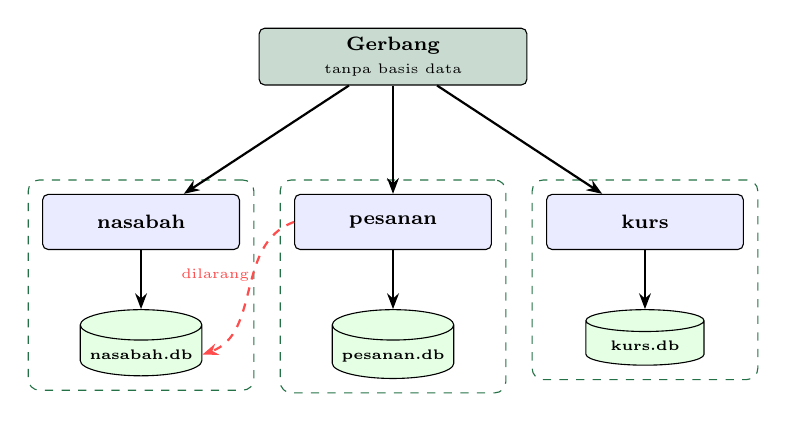
\begin{tikzpicture}[
        layanan/.style={draw, rounded corners=2pt, minimum width=2.5cm,
          minimum height=0.7cm, align=center, font=\scriptsize\bfseries},
        simpan/.style={draw, cylinder, shape border rotate=90, aspect=0.25,
          minimum height=0.6cm, minimum width=1.5cm, align=center,
          font=\tiny\bfseries},
        panah/.style={-{Stealth[length=2mm]}, thick},
        larangan/.style={-{Stealth[length=2mm]}, thick, dashed, red!70},
        batas/.style={draw, dashed, rounded corners=4pt, praditagreen,
          inner sep=5pt}
      ]
        \node[layanan, fill=blue!8] (nasabah) at (0,0) {nasabah};
        \node[layanan, fill=blue!8] (pesanan) at (3.2,0) {pesanan};
        \node[layanan, fill=blue!8] (kurs) at (6.4,0) {kurs};

        \node[simpan, fill=green!10, below=0.75cm of nasabah] (dbn)
          {nasabah.db};
        \node[simpan, fill=green!10, below=0.75cm of pesanan] (dbp)
          {pesanan.db};
        \node[simpan, fill=green!10, below=0.75cm of kurs] (dbk) {kurs.db};

        \draw[panah] (nasabah) -- (dbn);
        \draw[panah] (pesanan) -- (dbp);
        \draw[panah] (kurs) -- (dbk);

        \node[batas, fit=(nasabah)(dbn)] (bn) {};
        \node[batas, fit=(pesanan)(dbp)] (bp) {};
        \node[batas, fit=(kurs)(dbk)] (bk) {};

        \node[layanan, fill=praditagreen!25, minimum width=3.4cm] (gerbang)
          at (3.2,2.1) {Gerbang\\{\tiny\mdseries tanpa basis data}};

        \draw[panah] (gerbang) -- (nasabah);
        \draw[panah] (gerbang) -- (pesanan);
        \draw[panah] (gerbang) -- (kurs);

        \draw[larangan] (pesanan.west) to[out=200, in=20]
          node[font=\tiny, above left=-1pt and -4pt] {dilarang} (dbn.east);
      \end{tikzpicture}}
  \end{center}

  \vspace{2pt}
  {\small Garis putus-putus hijau adalah batas layanan sekaligus batas datanya.
  Panah merah adalah jalur yang dilarang.}
\end{frame}

\begin{frame}{{\Large Analogi: Unit Kegiatan Mahasiswa}}
  \vspace{10pt}
  \begin{itemize}\small
    \item Paduan suara, klub robotika, dan tim futsal memegang daftar
          anggotanya sendiri.
    \item Pengurus satu unit tidak pernah membuka daftar unit lain.
    \item Laporan mahasiswa yang aktif di lebih dari satu unit menuntut
          petugas meminta daftar dari setiap unit, lalu mencocokkannya
          sendiri.
    \item Imbalannya, tim futsal dapat mengubah bentuk daftarnya tanpa
          menunggu unit lain, dan unit yang libur tidak menghentikan unit
          lainnya.
  \end{itemize}

  \vspace{10pt}
  {\small Pekerjaan mencocokkan itulah kode penggabung di dalam gerbang.}
\end{frame}

\begin{frame}{{\Large Beda dari Service-Based}}
  \vspace{6pt}
  \centering
  \scriptsize
  \begin{tabularx}{0.96\textwidth}{|l|X|X|}
    \hline
    \textbf{Yang dibandingkan} & \textbf{\textit{Service-based}} & \textbf{Mikroservis} \\
    \hline
    Basis data & Satu, dipakai bersama seluruh layanan & Satu per layanan, tidak dipakai bersama \\
    \hline
    Penggabungan data & Satu kueri SQL dengan JOIN & Beberapa panggilan lalu digabung di dalam kode \\
    \hline
    Rilis satu layanan & Mungkin, selama skemanya tidak berubah & Mungkin, termasuk ketika skemanya berubah \\
    \hline
    Matinya satu layanan & Layanan lain tetap jalan, kecuali basis datanya ikut mati & Layanan lain tetap jalan, dan basis datanya terpisah \\
    \hline
    Ukuran layanan & Kasar, beberapa kemampuan besar & Halus, satu kemampuan per layanan \\
    \hline
  \end{tabularx}

  \vspace{6pt}
  \raggedright
  {\small Perbedaannya hanya satu baris, yaitu baris pertama, namun akibatnya
  terasa pada keempat baris lainnya.}
\end{frame}

\begin{frame}[fragile]{{\Large Monolit: Satu Kueri JOIN}}
  \vspace{4pt}
\begin{lstlisting}[style=SqlStyle]
SELECT n.nama, n.kota, n.rekening,
       p.id, p.mata_uang, p.nominal, k.dasar, k.margin
FROM nasabah AS n
JOIN pesanan AS p ON p.id_nasabah = n.id
JOIN kurs AS k ON k.mata_uang = p.mata_uang
WHERE n.id = ? AND p.status = ?
ORDER BY p.id
\end{lstlisting}

  \vspace{4pt}
  {\small Ketiga tabel berada di satu \textit{file}, sehingga mesin basis data
  mengerjakan penggabungannya sendiri. Seluruh laporan selesai dalam satu
  perjalanan ke basis data.}
\end{frame}

\begin{frame}[fragile]{{\Large Mikroservis: Gerbang Menggabungkan}}
  \vspace{2pt}
\begin{lstlisting}[style=PythonStyle]
nasabah = ambil_json(f"{alamat.NASABAH}/nasabah/{id_nasabah}", token)
if nasabah is None:
  return {"galat": "layanan nasabah tidak menjawab"}, 503
jawaban_pesanan = ambil_json(f"{alamat.PESANAN}/pesanan?nasabah={id_nasabah}")
if jawaban_pesanan is None:
  return {"galat": "layanan pesanan tidak menjawab"}, 503
daftar_pesanan = jawaban_pesanan["pesanan"]
kurs = kumpulkan_kurs(daftar_pesanan)
isi = [gabungkan_baris(satu, kurs[satu["mata_uang"]]) for satu in daftar_pesanan]
\end{lstlisting}

  \vspace{2pt}
  {\small Kueri JOIN tidak dapat ditulis, sebab ketiga tabel berada di tiga
  \textit{file}. Dua baris terakhir menggantikan klausa \texttt{JOIN}, dan
  pencocokannya menjadi tanggungan penulis gerbang.}
\end{frame}

\begin{frame}{{\Large \textit{Class Diagram}: Tiga Layanan}}
  \vspace{4pt}
  \begin{center}
    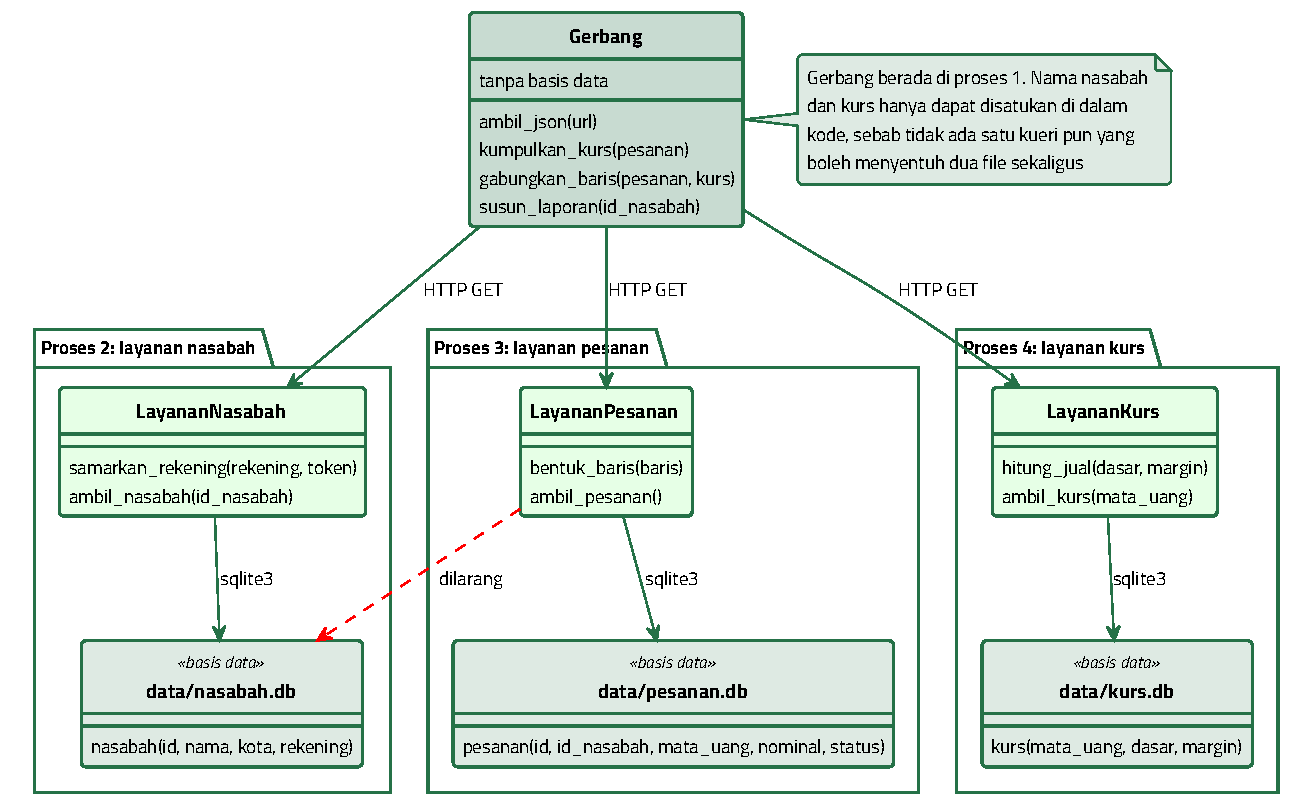
\includegraphics[width=\textwidth, height=0.72\textheight,
      keepaspectratio]{kelas-mikroservis.pdf}
  \end{center}
\end{frame}

\begin{frame}{{\Large Penjelasan \textit{Class Diagram}}}
  \vspace{10pt}
  \begin{itemize}\small
    \item Gerbang di sebelah kiri tidak memiliki basis data sama sekali.
    \item Ketiga layanan di tengah masing-masing memegang satu objek
          \texttt{Tabel} untuk satu \textit{file} SQLite.
    \item Setiap panah sqlite3 berhenti di dalam batas layanannya sendiri.
    \item Panah merah putus-putus adalah jalur yang dilarang, yaitu satu
          layanan membuka \textit{file} milik layanan lain.
  \end{itemize}

  \vspace{10pt}
  {\small Monolit memakai objek \texttt{Tabel} yang sama dengan ketiga
  layanan, sehingga isi datanya tidak mungkin berbeda.}
\end{frame}

\begin{frame}{{\Large \textit{Sequence Diagram}: Satu Laporan}}
  \vspace{4pt}
  \begin{center}
    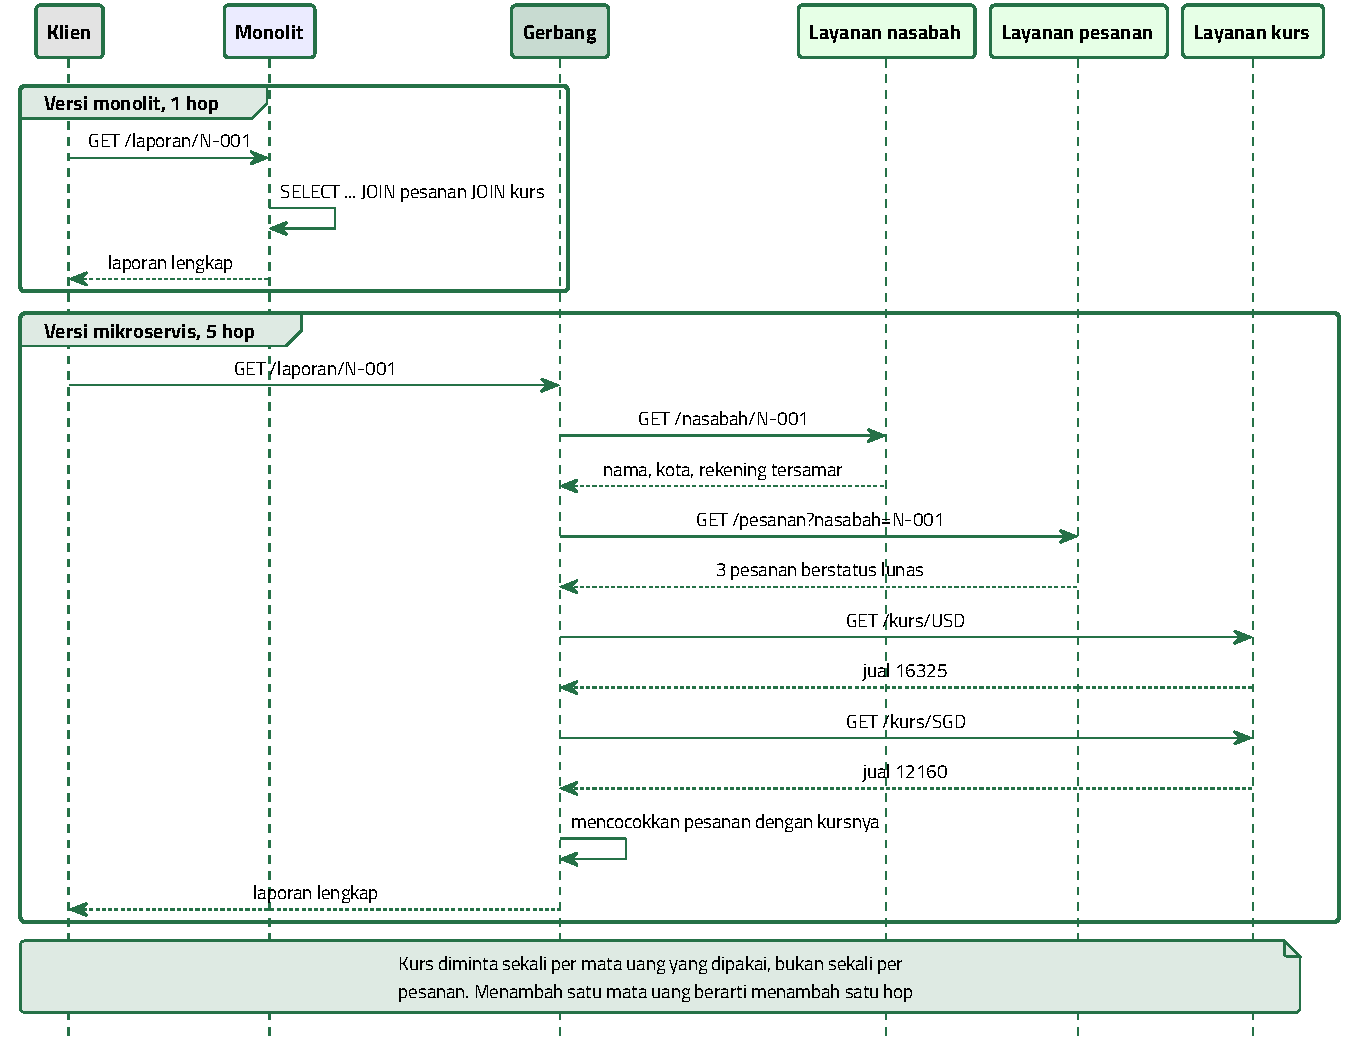
\includegraphics[width=\textwidth, height=0.74\textheight,
      keepaspectratio]{sekuens-mikroservis.pdf}
  \end{center}
\end{frame}

\begin{frame}{{\Large Penjelasan \textit{Sequence Diagram}}}
  \vspace{10pt}
  \begin{itemize}\small
    \item Monolit menjawab laporan nasabah N-001 dengan satu \textit{hop},
          yaitu dari klien ke prosesnya sendiri.
    \item Gerbang meminta data nasabah, lalu daftar pesanan, lalu kurs setiap
          mata uang yang muncul.
    \item Nasabah N-001 memiliki tiga pesanan lunas dalam dua mata uang,
          sehingga kurs diminta dua kali dan laporannya menempuh lima
          \textit{hop}.
    \item Kurs diminta sekali per mata uang, bukan sekali per pesanan, sebab
          hasilnya disimpan sementara selama laporan disusun.
  \end{itemize}

  \vspace{10pt}
  {\small Menambah satu mata uang baru pada pesanan tetap berarti menambah
  satu \textit{hop}.}
\end{frame}

\begin{frame}{{\Large Hasil: Harga Penggabungan}}
  \vspace{6pt}
  \centering
  \small
  \begin{tabularx}{0.8\textwidth}{|X|l|l|}
    \hline
    \textbf{Yang dibandingkan} & \textbf{Monolit} & \textbf{Mikroservis} \\
    \hline
    Median satu laporan & 1,63 ms & 7,53 ms \\
    \hline
    Persentil ke-95 & 1,96 ms & 8,47 ms \\
    \hline
    Terbesar & 2,39 ms & 9,28 ms \\
    \hline
    Baris kode penggabung & 26 & 44 \\
    \hline
    \textit{Request} jaringan & 1 & 5 \\
    \hline
    Putaran lebih cepat & 200 dari 200 & 0 dari 200 \\
    \hline
  \end{tabularx}

  \vspace{6pt}
  \raggedright
  {\small Dua ratus putaran. Isi kedua laporan sama persis sesudah \textit{key}
  \texttt{lompatan} dibuang, sehingga yang dibandingkan memang harganya.}
\end{frame}

\begin{frame}{{\Large Hasil: Latensi dan \textit{Hop}}}
  \vspace{6pt}
  \centering
  \small
  \begin{tabularx}{0.92\textwidth}{|l|X|l|l|l|l|}
    \hline
    \textbf{Versi} & \textbf{\textit{Request}} & \textbf{Median} & \textbf{p95} & \textbf{Terbesar} & \textbf{\textit{Hop}} \\
    \hline
    Monolit & nasabah & 1,60 ms & 1,85 ms & 2,16 ms & 1 \\
    \hline
    Monolit & laporan & 1,62 ms & 1,83 ms & 2,02 ms & 1 \\
    \hline
    Mikroservis & nasabah & 3,00 ms & 3,30 ms & 3,57 ms & 2 \\
    \hline
    Mikroservis & laporan & 7,77 ms & 8,43 ms & 9,18 ms & 5 \\
    \hline
  \end{tabularx}

  \vspace{6pt}
  \raggedright
  {\small Dua ratus putaran. Kedua versi menyala berbarengan dan diukur
  bergantian di dalam putaran yang sama.}
\end{frame}

\begin{frame}{{\Large Membaca Hasilnya}}
  \vspace{10pt}
  \begin{itemize}\small
    \item \textit{Request} nasabah menempuh satu \textit{hop} tambahan dan menjadi
          1,9 kali lebih lambat, dengan selisih median 1,40 ms.
    \item \textit{Request} laporan menempuh empat \textit{hop} tambahan dan menjadi
          4,8 kali lebih lambat, dengan selisih median 6,14 ms.
    \item Biaya mikroservis tumbuh mengikuti jumlah \textit{hop}, bukan
          mengikuti jumlah layanan yang terpasang.
    \item Layanan yang banyak tetapi jarang dipanggil bersama tidak mahal,
          sedangkan tiga layanan yang selalu dipanggil bersama sudah cukup
          mahal.
  \end{itemize}

  \vspace{10pt}
  {\small Kedua jalur dimenangkan monolit pada 200 dari 200 putaran, dan nilai
  terbesar paling jauh 1,35 kali mediannya.}
\end{frame}

\begin{frame}{{\Large Hasil: Layanan Kurs Mati}}
  \vspace{6pt}
  \centering
  \small
  \begin{tabularx}{0.86\textwidth}{|l|X|X|}
    \hline
    \textbf{\textit{Request}} & \textbf{Monolit, proses mati} & \textbf{Mikroservis, layanan kurs mati} \\
    \hline
    nasabah & gagal & penuh \\
    \hline
    kurs & gagal & gagal \\
    \hline
    laporan & gagal & sebagian \\
    \hline
    Terlayani & 0 dari 3 & 2 dari 3 \\
    \hline
  \end{tabularx}

  \vspace{6pt}
  \raggedright
  {\small Golongan sebagian berarti laporannya tetap keluar dengan nilai rupiah
  kosong dan \textit{key} \texttt{lengkap} bernilai \texttt{false}. Pilihan itu
  ditulis sebagai sembilan baris di dalam gerbang.}
\end{frame}

\begin{frame}{{\Large Kasus: Penyedia Kurs Terganggu}}
  \vspace{8pt}
  \begin{enumerate}\small
    \item Sebuah bank memindahkan sistem penukaran valuta asingnya ke
          mikroservis.
    \item Pada bulan pertama, penyedia kurs pihak ketiga terganggu selama
          empat puluh menit, dan layanan kurs ikut berhenti menjawab.
    \item Gerbangnya menolak menyusun laporan tanpa kurs, sehingga seluruh
          halaman riwayat menampilkan \textit{error}.
    \item Petugas cabang tidak dapat melihat pesanan yang sudah lunas, padahal
          daftar itu tidak membutuhkan kurs.
    \item Sesudah gerbangnya diubah, gangguan serupa pada bulan berikutnya
          hanya menghilangkan satu kolom.
  \end{enumerate}

  \vspace{6pt}
  {\small Setiap pemanggilan antar layanan karena itu butuh tenggang waktu,
  penanganan \textit{error}, dan keputusan tentang apa yang terjadi
  sesudahnya.}
\end{frame}

\begin{frame}{{\Large Hasil: Rilis Ulang Layanan Kurs}}
  \vspace{6pt}
  \centering
  \small
  \begin{tabularx}{0.9\textwidth}{|l|X|l|l|l|}
    \hline
    \textbf{Versi} & \textbf{Lalu lintas} & \textbf{Tidak penuh} & \textbf{Padam} & \textbf{Padam terbesar} \\
    \hline
    Monolit & nasabah & 7 dari 200 & 198 ms & 225 ms \\
    \hline
    Monolit & laporan & 7 dari 200 & 196 ms & 207 ms \\
    \hline
    Mikroservis & nasabah & 0 dari 200 & 186 ms & 232 ms \\
    \hline
    Mikroservis & laporan & 9 dari 200 & 237 ms & 247 ms \\
    \hline
  \end{tabularx}

  \vspace{6pt}
  \raggedright
  {\small Median tujuh kali rilis. Dua ratus \textit{request} berjarak tetap
  25 ms, dan rilisnya dipicu pada \textit{request} kelima puluh.}
\end{frame}

\begin{frame}{{\Large Membaca Hasil Rilis}}
  \vspace{10pt}
  \begin{itemize}\small
    \item Merilis kurs pada mikroservis tidak mengganggu satu pun \textit{request}
          nasabah, walaupun prosesnya mati sekitar dua ratus milidetik.
    \item Pada monolit, 7 dari 200 \textit{request} nasabah ikut gagal, padahal
          nasabah tidak berhubungan dengan kurs.
    \item Kolom padam pada keempat baris berdekatan, sebab yang dinyalakan
          ulang sama-sama satu proses Python berisi satu aplikasi Flask.
  \end{itemize}

  \vspace{10pt}
  {\small Yang berbeda bukan lama padamnya, melainkan siapa saja yang ikut
  padam.}
\end{frame}

\begin{frame}{{\Large Kapan Sepadan}}
  \vspace{6pt}
  \centering
  \scriptsize
  \begin{tabularx}{0.96\textwidth}{|X|X|}
    \hline
    \textbf{Sepadan ketika} & \textbf{Belum sepadan ketika} \\
    \hline
    Tiap layanan umumnya melayani \textit{request}-nya sendiri & Hampir setiap halaman membutuhkan tiga layanan sekaligus \\
    \hline
    Irama perubahan tiap bagian jauh berbeda & Seluruh bagian berubah bersama-sama pada rilis yang sama \\
    \hline
    Batas domainnya sudah terbukti dipakai & Batasnya masih ditebak dan sering berpindah \\
    \hline
    Padamnya satu bagian tidak boleh menjatuhkan bagian lain & Sistemnya memang mati bersama-sama tanpa merugikan siapa pun \\
    \hline
  \end{tabularx}

  \vspace{6pt}
  \raggedright
  {\small Fowler menyarankan sistem baru dimulai sebagai monolit, sebab batas
  yang benar hampir selalu baru terlihat sesudah sistemnya dipakai.}
\end{frame}

\begin{frame}{{\Large Kasus: Dipecah Terlalu Dini}}
  \vspace{8pt}
  \begin{enumerate}\small
    \item Sebuah tim membangun sistem pembayaran kampus langsung sebagai enam
          layanan, sebelum domainnya dipahami.
    \item Batas antara layanan tagihan dan layanan pembayaran ternyata keliru,
          sebab satu tagihan boleh dicicil.
    \item Memindahkan satu tabel menuntut pemindahan data, dua kali rilis, dan
          satu perubahan kontrak yang disepakati dua tim.
    \item Pekerjaan yang pada satu basis kode berupa pemindahan satu kelas
          menjadi pekerjaan tiga pekan.
    \item Pada akhir semester, empat dari enam layanan disatukan kembali.
  \end{enumerate}
\end{frame}

\begin{frame}{{\Large \textit{Summary}}}
  \vspace{8pt}
  \begin{itemize}\small
    \item Setiap layanan memegang basis datanya sendiri, dan aturan itulah
          yang membedakannya dari \textit{service-based architecture}.
    \item Penggabungan pindah ke gerbang, sehingga laporan menempuh lima
          \textit{hop} melawan satu dan menjadi 4,8 kali lebih lambat.
    \item Layanan kurs yang mati hanya menghilangkan kolom rupiah, yaitu dua dari
          tiga \textit{request} tetap terlayani melawan nol dari tiga.
    \item Merilis kurs tidak mengganggu satu pun \textit{request} nasabah,
          sedangkan monolit menggagalkan 7 dari 200.
  \end{itemize}

  \vspace{8pt}
  {\small Batas layanan dan batas data harus ditarik
  bersamaan. Karena itu banyak sistem sebaiknya dimulai sebagai monolit, lalu
  dipecah sesudah batasnya terbukti.}
\end{frame}

\begin{frame}[fragile]{{\Large Persiapan Latihan}}
  \vspace{5pt}
\begin{lstlisting}[language=bash]
bash sources/siapkan_venv.sh
source .venv/bin/activate
cd sources/chapter13
python basis_data.py
# layanan_nasabah  data/nasabah.db   1 tabel, 3 baris
python penjalan.py mikroservis
# Versi mikroservis menyala, 4 proses.
\end{lstlisting}

  \vspace{6pt}
  {\small Bab ini memakai Flask dan requests, dan \textit{port} 5300 beserta
  5310 sampai 5313 harus kosong. Langkah lengkap, tabel contoh, dan lembar
  isian ada di buku, Bab 13, yang menjadi rujukan utama latihan ini.}
\end{frame}

\begin{frame}[fragile]{{\Large Latihan 1: Latensi dan \textit{Hop}}}
  \vspace{2pt}
  {\small Tujuan: membuktikan bahwa biayanya mengikuti jumlah \textit{hop}.}

  \vspace{2pt}
\begin{lstlisting}[language=bash, basicstyle=\ttfamily\tiny]
python ukur_latensi.py
# Jalur nasabah  monolit lebih cepat : 200 dari 200, selisih median   1.40 ms, 1.9 kali
# Jalur laporan  monolit lebih cepat : 200 dari 200, selisih median   6.14 ms, 4.8 kali
\end{lstlisting}

  \vspace{2pt}
  \begin{enumerate}\small
    \item Catat keempat baris hasil beserta dua baris pencacahannya.
    \item Temukan baris yang menghitung \textit{key} \texttt{lompatan} pada
          \texttt{susun\_laporan} di \texttt{gerbang.py}.
    \item Panggil \texttt{/laporan/N-002} pada versi mikroservis, lalu catat
          jumlah \textit{hop}-nya.
  \end{enumerate}

  \vspace{2pt}
  {\small Pertanyaan: berapa biaya rata-rata satu \textit{hop}, dan apakah
  biaya itu menjelaskan baris laporan?}
\end{frame}

\begin{frame}[fragile]{{\Large Latihan 2: Harga Penggabungan}}
  \vspace{2pt}
  {\small Tujuan: mengukur harga yang dibayar karena basis datanya terpisah.}

  \vspace{2pt}
\begin{lstlisting}[language=bash]
python ukur_laporan.py
# Median laporan mikroservis        : 7.53 ms
# Baris kode penggabung mikroservis : 44
# Request jaringan mikroservis      : 5
\end{lstlisting}

  \vspace{2pt}
  \begin{enumerate}\small
    \item Catat kedua belas baris laporannya.
    \item Bandingkan \texttt{KUERI\_LAPORAN} dengan \texttt{susun\_laporan}.
    \item Tambahkan satu pesanan JPY untuk N-001 beserta kursnya, lalu
          jalankan ulang kedua skrip dan catat \textit{request} jaringannya.
  \end{enumerate}

  \vspace{2pt}
  {\small Pertanyaan: mengapa jumlah \textit{request} jaringan naik pada
  mikroservis tetapi tidak pada monolit?}
\end{frame}

\begin{frame}[fragile]{{\Large Latihan 3: Rilis Ulang}}
  \vspace{2pt}
  {\small Tujuan: mengukur imbalan rilis yang berdiri sendiri.}

  \vspace{2pt}
\begin{lstlisting}[language=bash]
python uji_kegagalan.py
# Terlayani sesudah kurs mati, mikroservis : 2 dari 3
python ukur_rilis.py
# mikroservis  nasabah      200         0      0           0       186       232
\end{lstlisting}

  \vspace{2pt}
  \begin{enumerate}\small
    \item Catat hasil kedua skrip.
    \item Ubah \texttt{gabungkan\_baris} agar melempar \textit{error} ketika
          kursnya \texttt{None}.
    \item Jalankan ulang kedua skrip, catat perubahan golongan laporannya,
          lalu kembalikan kodenya.
  \end{enumerate}

  \vspace{2pt}
  {\small Pertanyaan: dengan menggabungkan ketiga latihan, apakah sistem ini
  sebaiknya dipecah sehalus ini?}
\end{frame}

\end{document}
